\documentclass[../report.tex]{subfiles}
\begin{document}
\graphicspath{{img/}{../img/}}



%\section{Overview}

%\todo{Add section intro}

%\begin{figure}
%\centering
%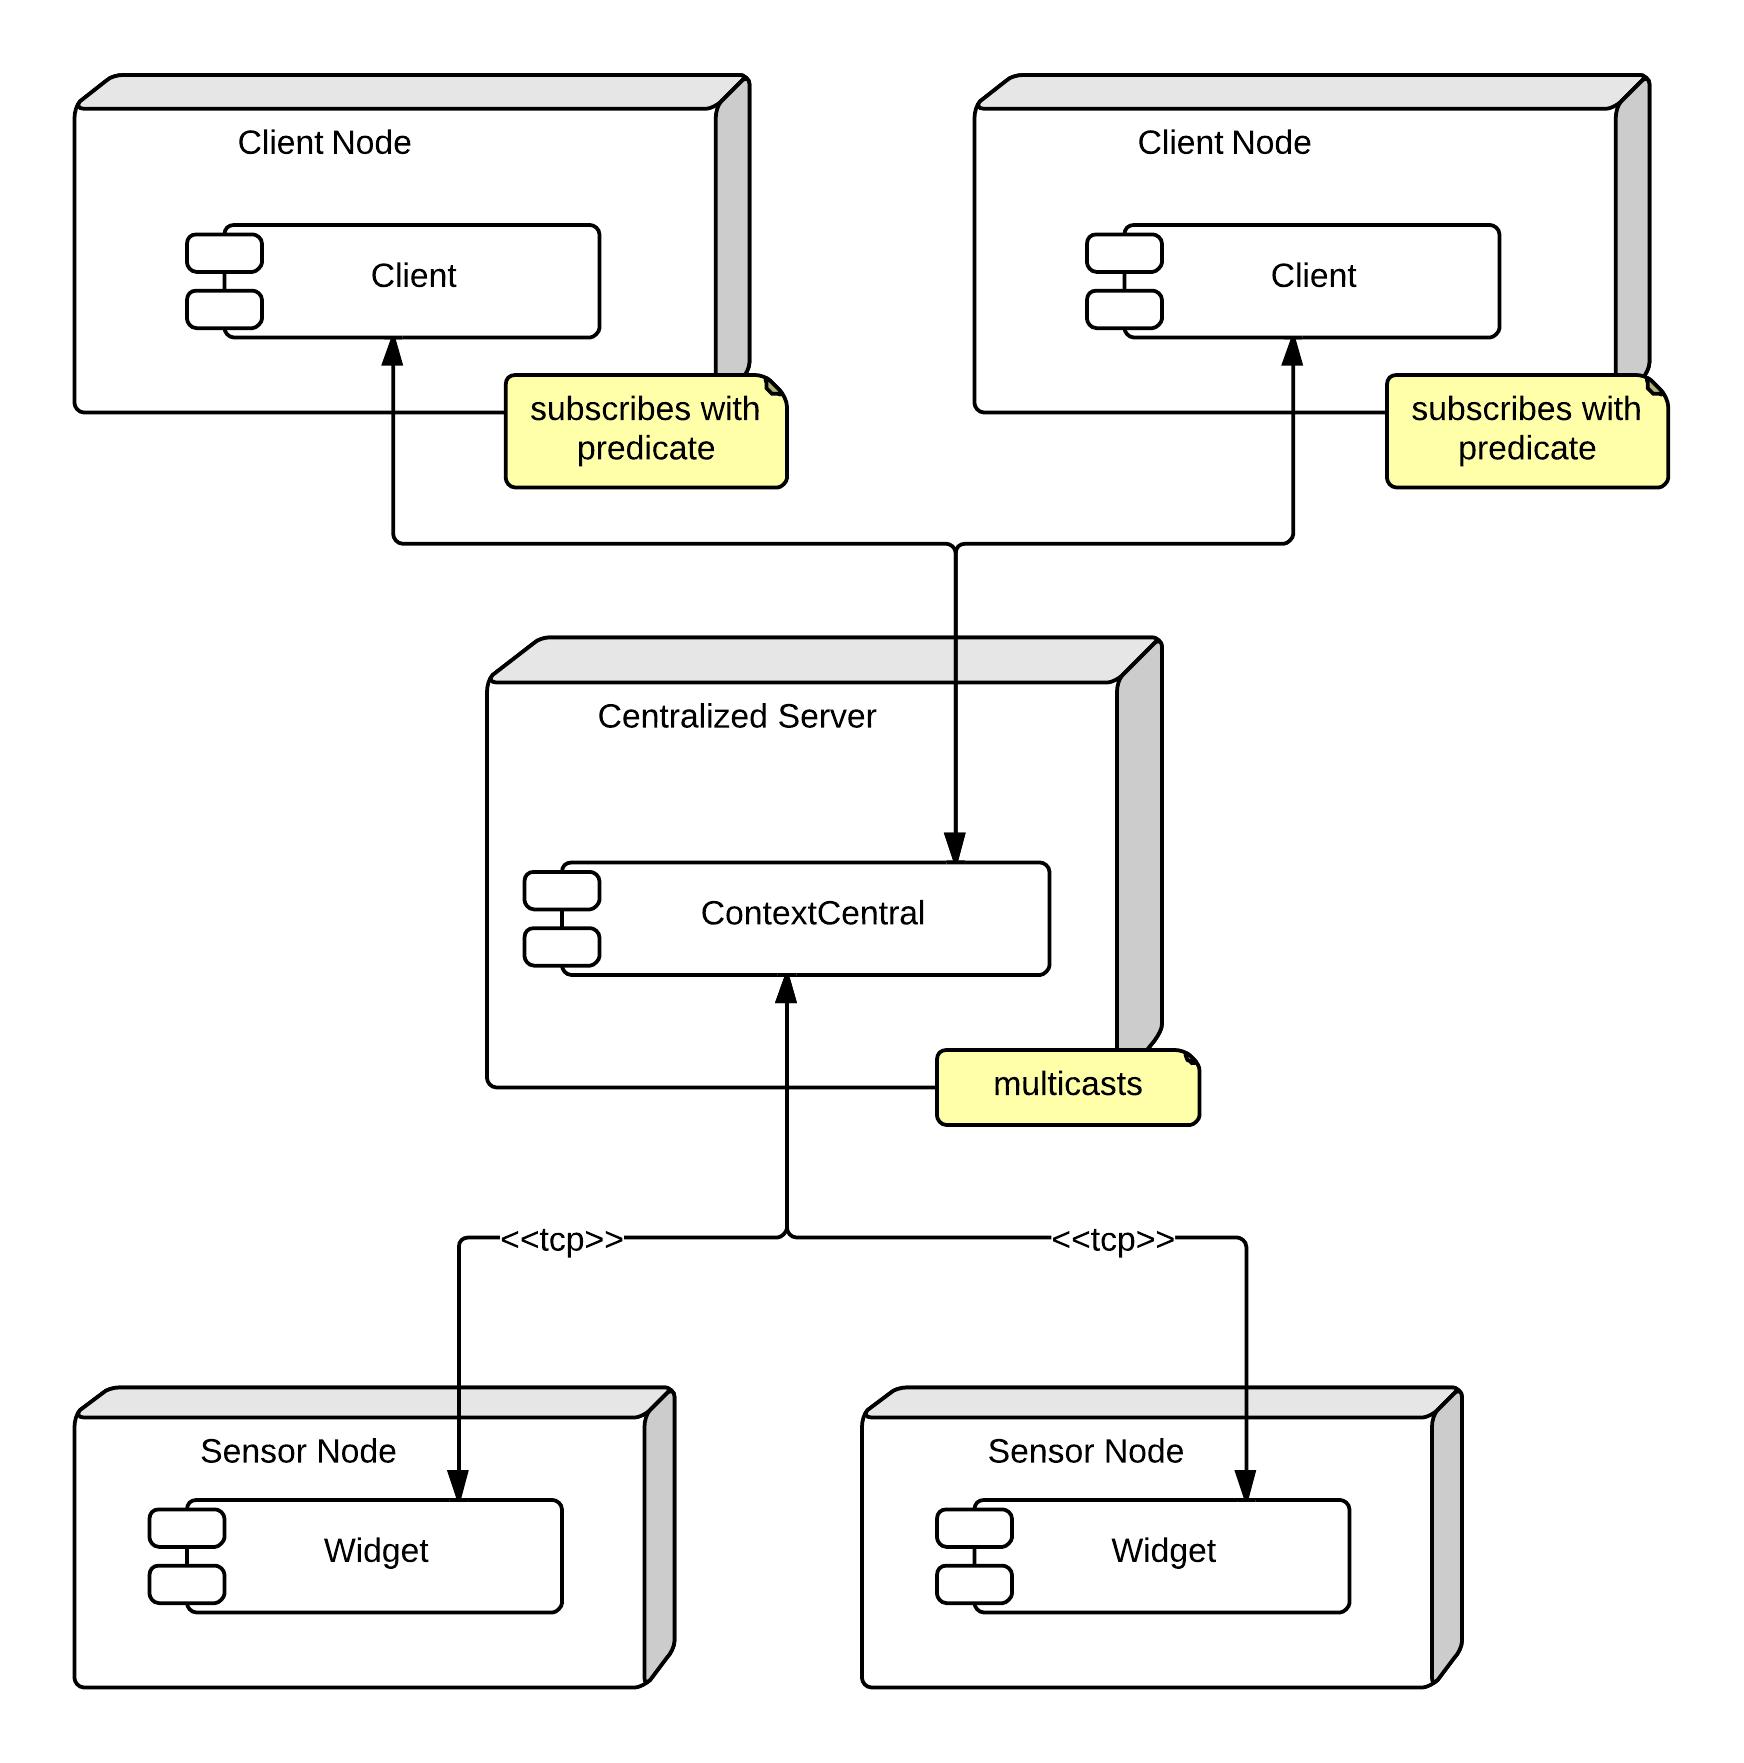
\includegraphics[width=\linewidth]{ComponentDiagram.png}
%\caption{OCon component decomposition}
%\label{fig:componentdiagram}
%\end{figure}


%\paragraph{The Client} is an observer interested in sensor data. It subscribes to a situation on the ContextCentral.

%\paragraph{The Widget} wraps a sensor and translates the raw data to entities which are sent to the ContextCentral.

%\paragraph{The ContextCentral} is the central for entity information and situations. When an entity is received from a widget it is saved to the central and all situations are checked and subscribers notified if their statuses changed due to the update.



\section{Encapsulation of Context}

Entities are generalized by the interface IEntity, specifying general information for all entities. AbstractEntity extends on IEntity and overrides ToString() with a meaningful implementation. Both are public and it is up the an implementor which to extend.

On figure \ref{fig:PersonImplementation} is extended a Person with property present motivated by the need for this context information.


\begin{figure}[H]
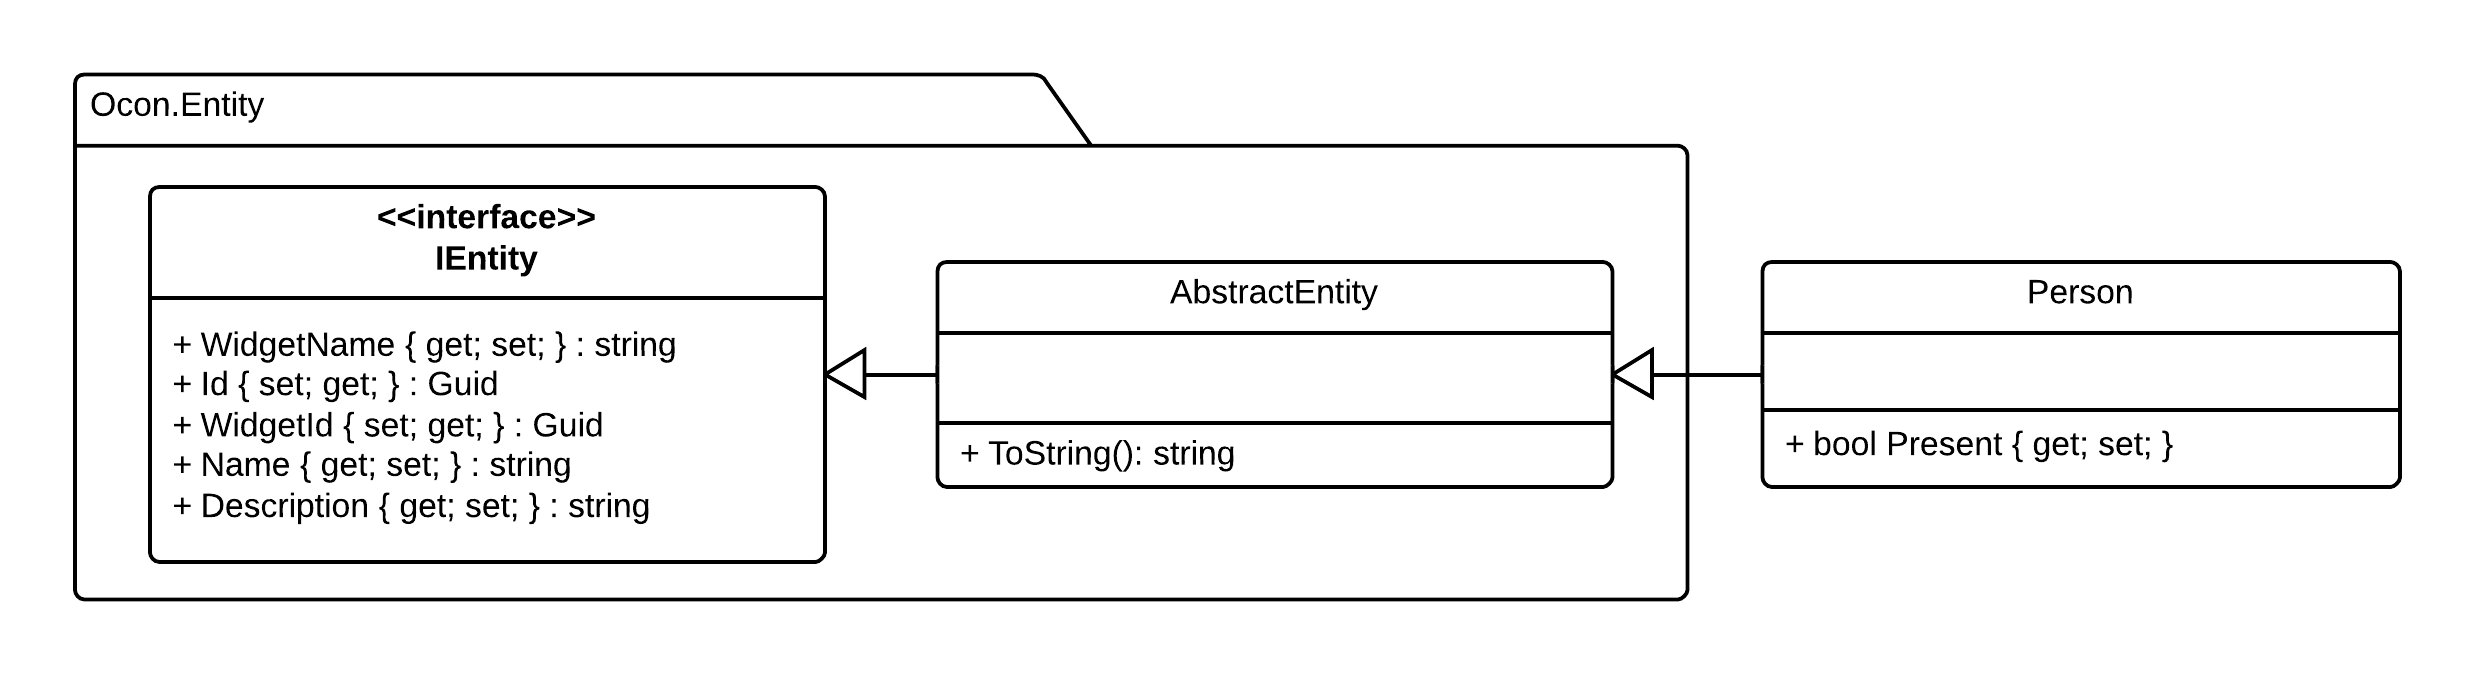
\includegraphics[width=\linewidth]{customEntityClass.png}
\caption{Person as a custom IEntity implementation}
\label{fig:PersonImplementation}
\end{figure}



\section{Situation predicate evaluation}
\todo{Short on how we evualate predicates}

\section{Widget}

The widget's purpose is to track entities and keep them updated in the central. The widget developer should translate sensor input to entities and then the OCon widget will facilitate tracking the entity and sending it to the central. (See figure \ref{seqwidget})

When the widget is notified about an entity from the sensor first it's checked weather or not the entity is already tracked by the widget. If not tracked it will be allocated a new GUID before it is sent to the central. The GUID is a unique ID used for distributed systems and allows OCon to distinguish between adding the entity as a new entity or updating an entity already know to the framework.

\begin{figure}
\centering
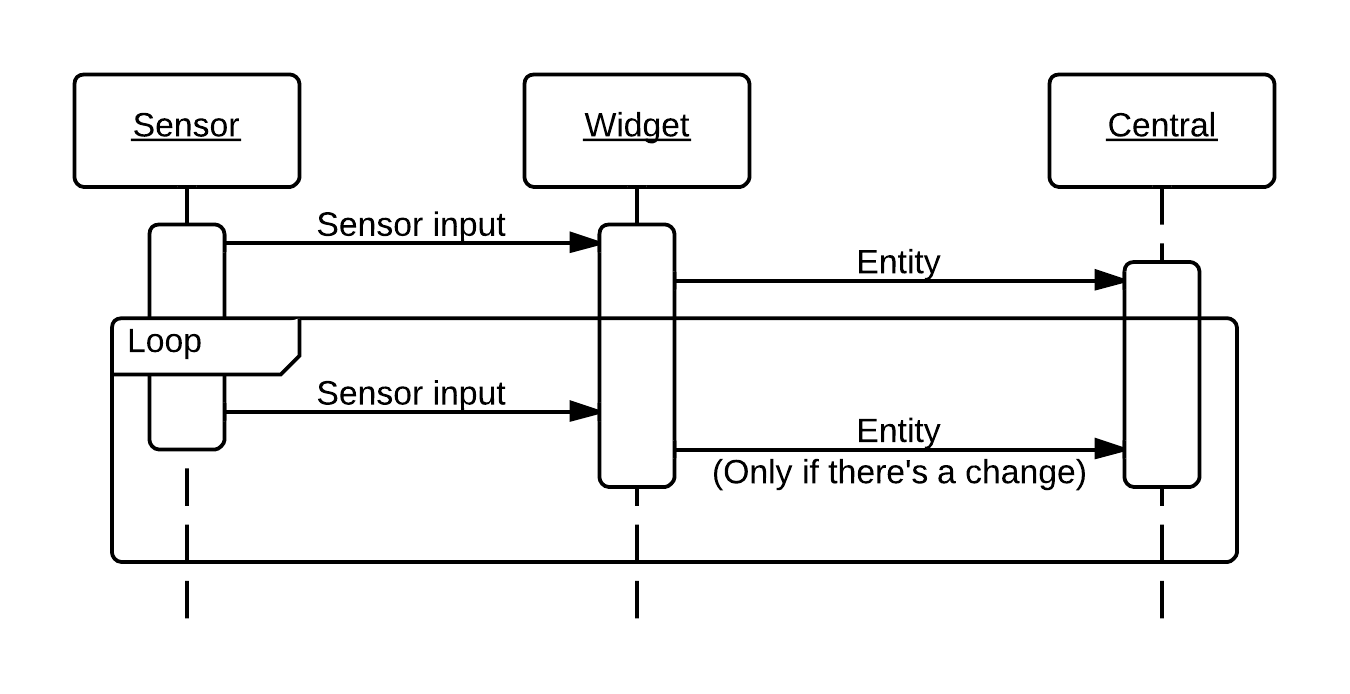
\includegraphics[width=\linewidth]{sequencediagram-widget.png}
\caption{Information flow from Widget to central}
\label{fig:seqwidget}
\end{figure}


\section{Central}
\todo{Write about the central}

\section{Client}

The client's purpose it to sent predicates to the central for tracking. When a situation update is sent from the central the client must be able to notify the parent application about the situation update. (See figure \ref{seqclient})

\begin{figure}
\centering
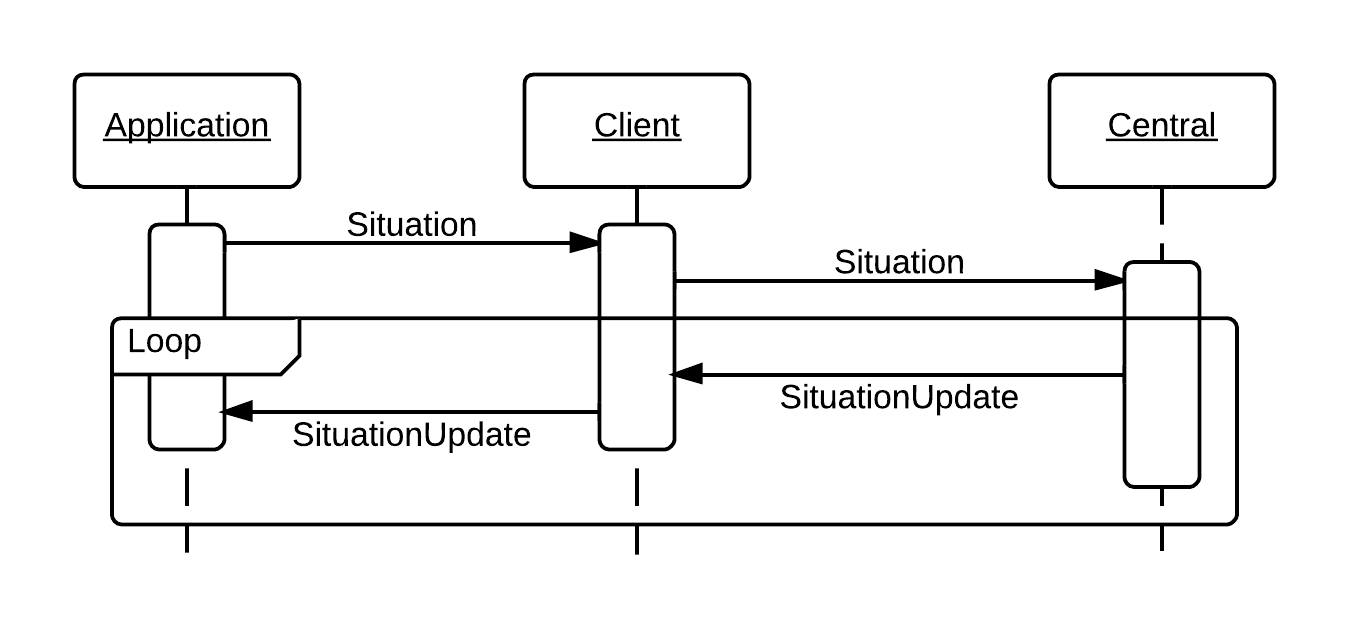
\includegraphics[width=\linewidth]{clientsequencediagram.png}
\caption{Information flow between client and central}
\label{fig:seqclient}
\end{figure}

When the central is discovered the client will sent its situations to the central. The central will compute the situation state and sent it back. Whenever the situation state changes the central will sent an update to the client containing the situations new state. The client will then fire an event which the application can listen and react to.

\section{Communication}

To supoort the design decision that the communication part should be injectable the communication have been interfaced.

OCon will contain a default communication implementation build using the TCP/IP layer. For serialization we have chosen to use json. These decisions have been made so that developers are not bound to the .NET platform and can make clients and widgets in other languages like Java, or C directly on a micro controllers like Arduino.

For peer discovery we have chosen to use IP multicast. The central will broadcast itself for peers to discover. The peer, clients and widgets, will be listening on the multicast endpoint and will invoke an event when a central is discovered.

The communication subsystem is a vital part of OCon as all communication between peers will go though the subsystem. See figure \ref{fig:widgetComHelper} and \ref{fig:clientComHelper} for a detailed view of the communication between client and central and widget and central.

Just like entities, peers are assigned a GUID. The GUID is an unique identifier for the peer and the communication class stores the IPEndPoints associated with the GUIDs. By doing this messages can be sent only by using the GUID and not the IPEndPoint which adds an abstraction layer to the subsystem.

To support clients being able to sent predicates to the central we must be able to serialize Predicates, but this is unfortunately not supported in .NET. Frameworks for handling the serialization have been researched, but none of the investigated frameworks was able serialize the predicates in OCon as custom types are used. Therefore serializing the predicate was forced out of scope. Instead of sending the predicate, predicates is hard coded in the central. The client can then subscribe them by sending a predicate identifier. This limits the usage of OCon, but it was not possible to include this feature in this project. A framework for serializing the predicates as expression trees should be doable, but that project is left for a later iteration of OCon.

\begin{figure}
\centering
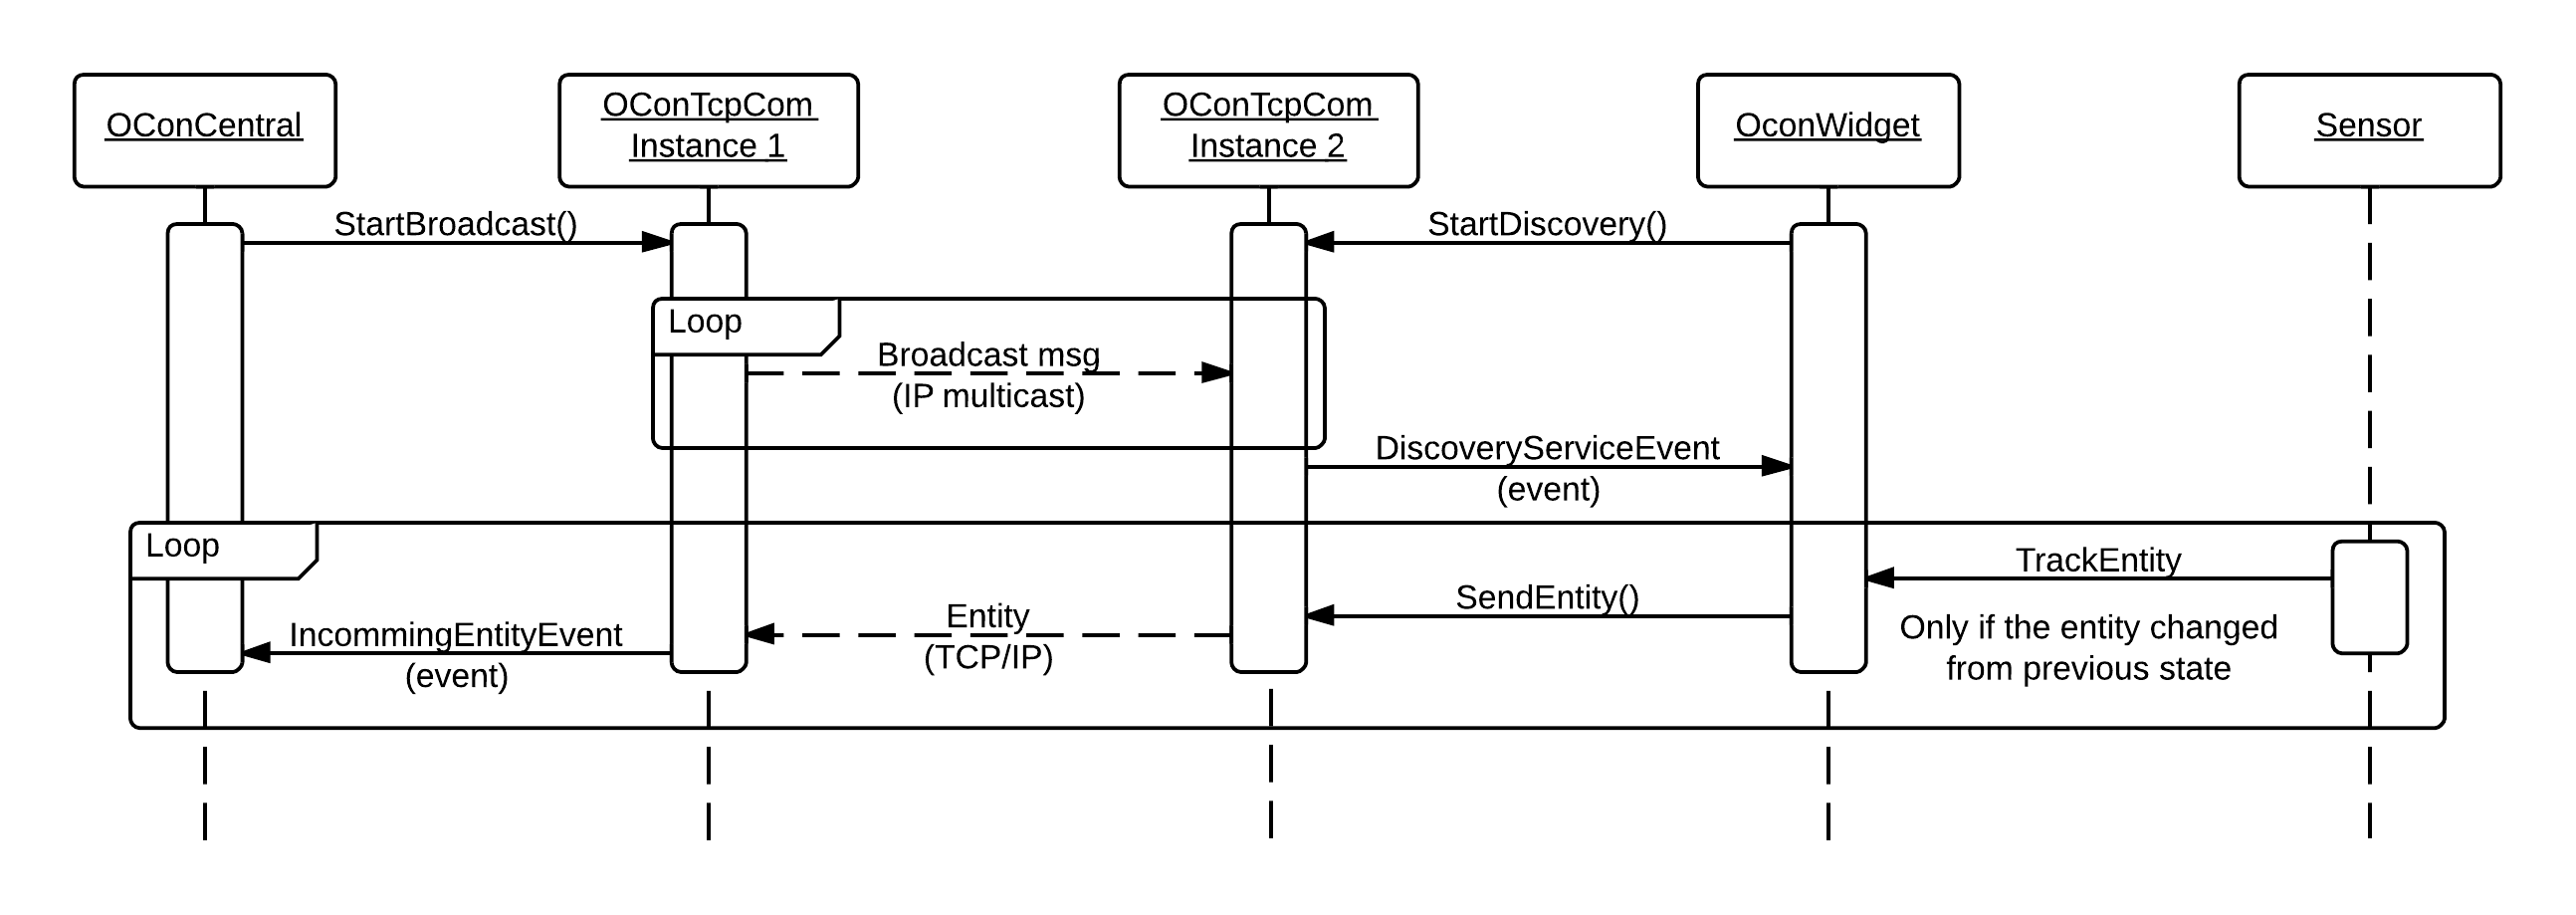
\includegraphics[width=\linewidth]{comHelperSequence-widget.png}
\caption{Widget to Central sequence diagram}
\label{fig:widgetComHelper}
\end{figure}

\begin{figure}
\centering
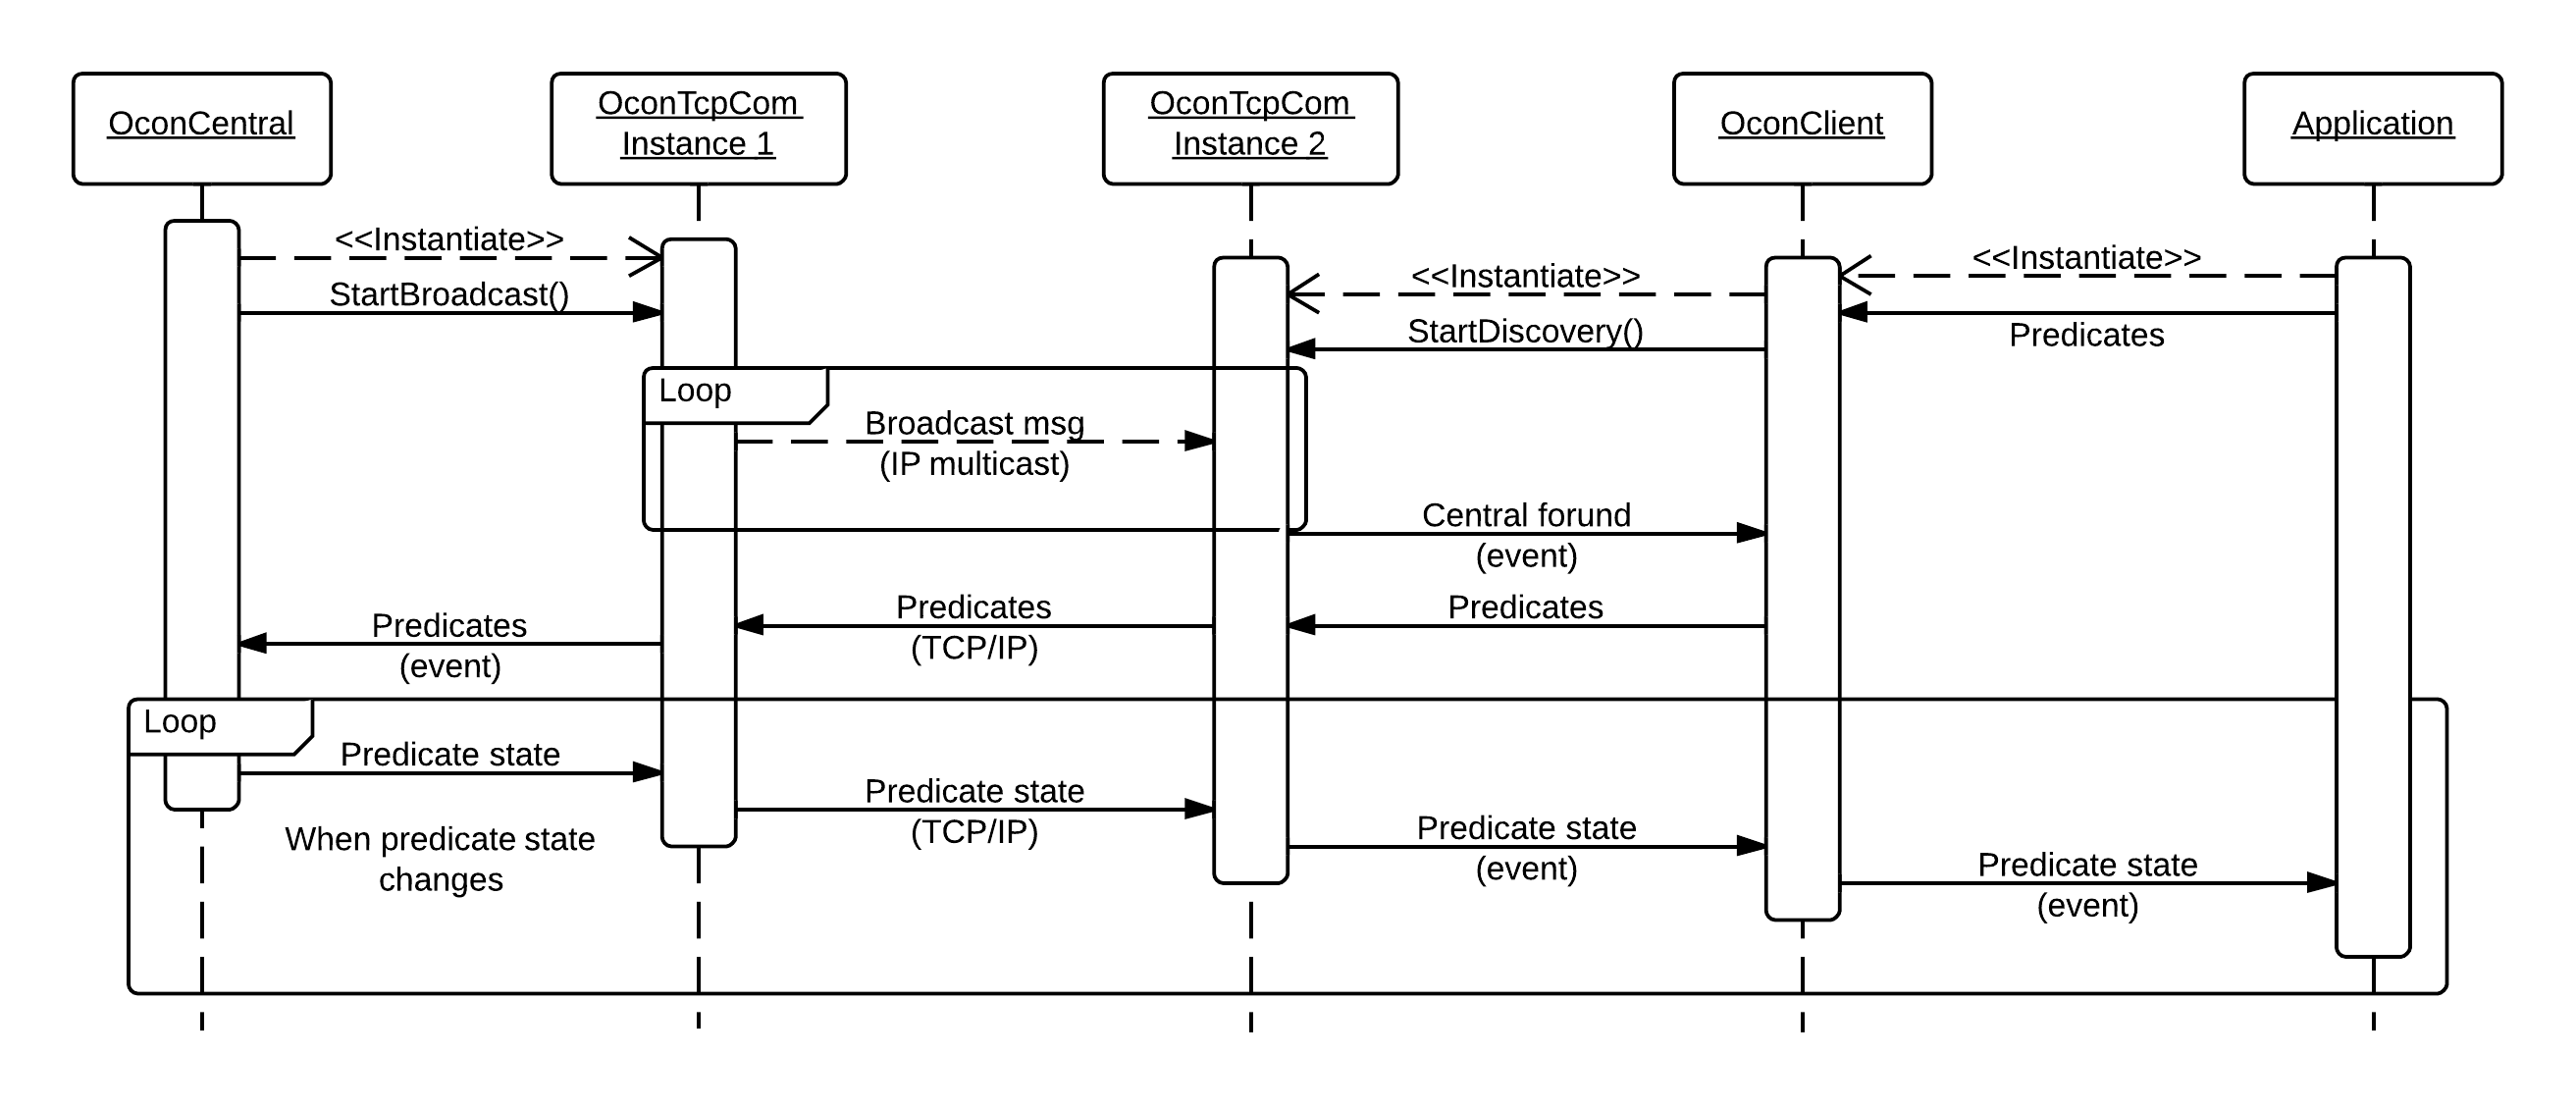
\includegraphics[width=\linewidth]{comHelperSequence-client.png}
\caption{Client to Central sequence diagram}
\label{fig:clientComHelper}
\end{figure}



\end{document}